\documentclass[11pt,a4paper]{article}
\usepackage[utf8]{inputenc}
\usepackage[spanish]{babel}
\usepackage{amsmath}
\usepackage{amsfonts}
\usepackage{amssymb}
\usepackage{graphicx}
\usepackage{geometry}
\usepackage{booktabs}
\geometry{margin=2.5cm}

\title{Informe de Prácticas: Resolución Numérica de la Ecuación de Schrödinger}
\author{Miguel Enterría Lastra \\ \small Métodos Numéricos y sus Aplicaciones a la Física}
\date{\today}

\begin{document}

\maketitle

\section{Objetivos}
El objetivo de esta práctica es encontrar la solución numérica de la ecuación de Schrödinger independiente del tiempo para el problema del pozo de potencial cuadrado y finito. Se compararán dos aproximaciones numéricas: el método de diferencias finitas y el método de Numerov.

\section{Fundamentos Teóricos}
La ecuación de Schrödinger unidimensional para una partícula no relativista es:
\begin{equation}
-\frac{\hbar^{2}}{2m}\frac{d^{2}\psi(x)}{dx^{2}}+V(x)\psi(x)=E\psi(x)
\end{equation}
Para su resolución numérica, reordenamos la ecuación como $y'' = f(x)y$:
\begin{equation}
\frac{d^{2}\psi(x)}{dx^{2}}=\frac{2m}{\hbar^{2}}(V(x)-E)\psi(x)
\end{equation}

\section{Metodología Numérica}

\subsection{Método de Diferencias Finitas}
Se basa en la discretización del espacio en pasos constantes $x_{i+1} = x_i + s$. Utilizando una aproximación de Taylor de orden $\mathcal{O}(\Delta^2 x)$, las ecuaciones de iteración son:
\begin{itemize}
    \item $\psi_{i+1} \approx \psi_i + \psi'_i \cdot \Delta x$
    \item $\psi'_{i+1} \approx \psi'_i + \frac{2m}{\hbar^2}(V_i - E)\psi_i \cdot \Delta x$
\end{itemize}

\subsection{Método de Numerov}
Este método ofrece una precisión de orden $\mathcal{O}(\Delta^6 x)$. Definimos la función auxiliar $\phi_k = \psi_k [1 - \frac{\Delta x^2 f_k}{12}]$. El algoritmo de integración sigue la relación:
\begin{equation}
\phi_{k+1} = 2\phi_k - \phi_{k-1} + \Delta x^2 f_k \psi_k
\end{equation}
donde $\psi_k = \phi_k / (1 - \frac{\Delta x^2 f_k}{12})$ y $f_k = \frac{2m}{\hbar^2}(V_k - E)$.

\subsection{Método de Disparo (Shooting Method)}
Para encontrar los autovalores de energía $E_n$, se utiliza el método de bisección. Se integra la función de onda para diferentes energías buscando aquellas que cumplen la condición de contorno en el infinito: $\psi(x \to \infty) = 0$.

Para esta solución primero se aplica un barrido inicial con un paso grande para detectar las zonas de cambio de signo donde luego se aplica el método de bisección.

\subsection{Comapración de métodos}

Ambos métodos dan resultados bastante parecidos que serán discutidos más adelante. Las principales diferencias de estos dos métodos son las que siguen:
\begin{enumerate}
    \item El método de diferencias finitas es dependiente de la paridad; por ello se buscan las soluciones pares e impares por separado. Aplicando las condiciones de contorno necesarias en cada caso.
    \item El orden de precisión del método de Numerov es mayor.
    \item Debido al anterior punto la velocidad de convergencia del método será mayor para el método de Numerov.
    \item Las condiciones de contorno para el método de diferncias finitas consistirán en valores para la función y su derivada en $x = 0$ y para Numerov en la suposición inicial del valor de la función en $-\infty$ (aproximando a un valor del espacio alejado del potencial) es cero y el siguiente valor muy bajo.
\end{enumerate}

Para ambos métodos la suposición para resolver es la misma: EL valor de la función en el inifinito es 0. En este caso se realiza esta suposición en un punto suficientemente alejado de la barrera de potencial.

Ambos métodos son dependientes del espaciado de nuestros puntos lo cual permitirá mayor precisión a la hora de encontrar la solución.

\subsection{Valores numéricos}
Se utilizaron variables adimensionales $u = x/a$, $k = \frac{2ma^2 V_0}{\hbar^2}$ y $\alpha = E/V_0$. Las condiciones iniciales para el estado fundamental (par) fueron $\psi(0)=1$ y $\psi'(0)=0$ y (impar) $\psi(0)=0$ y $\psi'(0)=1$ para el método de diferencias finitas. 
Para el método de Numerov, la elección del segundo valor de la función de onda se discutirá más adelante.

Para ambos casos se ha cogido un valor máximo de u de 2, ya que por encima de este valor empieza a dar problemas de convergencia del método. Para corregir estos problemas hay que reducir mucho el espaciado, lo que aumenta considerablemente el tiempo de computación.

Los valores numéricos de las constantes utilizadas, basados en las propiedades del sistema físico, son los siguientes:

\begin{itemize}
    \item \textbf{Anchura del pozo ($a$):} $1\,\text{\AA} = 10^{-10}\,\text{m}$.
    \item \textbf{Profundidad del pozo ($V_0$):} $244\,\text{eV}$.
    \item \textbf{Masa del electrón ($m_e$):} $0.511\,\text{MeV}/c^2$.
    \item \textbf{Constante de Planck reducida ($\hbar$):} $6.582 \times 10^{-16}\,\text{eV}\cdot\text{s}$.
    \item \textbf{Parámetro adimensional ($k$):} $64.0447$.
\end{itemize}

\section{Resultados: Pozo de Potencial Cuadrado}

Para la comparativa de los resultados se han obtenido los valores de la solución analítica a partir de la resolución presentada en el libro \textit{Quantum Physics of Atoms, Molecules, Solids, Nuclei, and Particles} (Second Edition) de Robert Eisberg y Robert Resnick.

En el caso del potencial estudiado, se obtienen tres estados ligados cuyos autovalores de energía cumplen la condición $E < V_0$. Estas soluciones se dividen en dos funciones de onda de simetría par y una de simetría impar. Los valores analíticos para el parámetro adimensional $\alpha$ se presentan en la siguiente tabla:

\begin{table}[h]
\centering
\begin{tabular}{c c c c}
\toprule
Estado ($n$) & Paridad & Expresión Analítica ($E$) & Valor de $\alpha$ ($E/V_0$) \\
\midrule
1 & Par & $\approx 0.0980 V_0$ & 0.0980 \\
2 & Par & $\approx 0.808 V_0$ & 0.8080 \\
3 & Impar & $\approx 0.383 V_0$ & 0.3830 \\
\bottomrule
\end{tabular}
\caption{Valores analíticos de los autovalores de energía para los estados ligados del pozo de potencial cuadrado.}
\end{table}

Una vez aplicado el método correspondiente se obtiene una lista de valores de la función $\psi(x)$ en el punto $U_{\max}$, el último punto de integración. Sobre esta lista se aplica el método de bisección.

\begin{figure}[h]
    \centering
    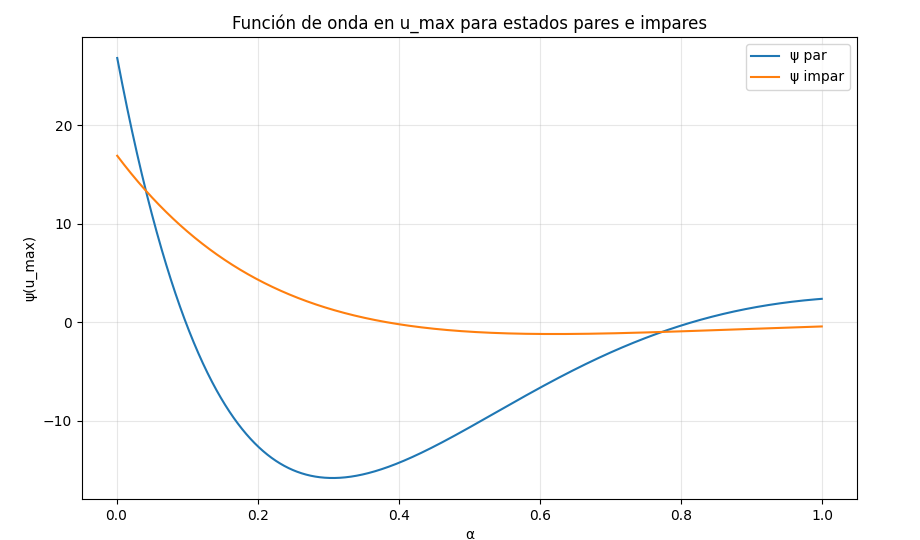
\includegraphics[width=0.8\textwidth]{imagenes/PsiUmax.png}
    \caption{Valor de $\psi(U_{\max})$ en función de la energía adimensional $\alpha$, utilizado para localizar intervalos de cambio de signo y aplicar posteriormente bisección en el método de diferencias finitas.}
    \label{fig:psi_umax}
\end{figure}

\subsection{Método de diferencias finitas}

Se va a realizar una comparación de los distintos valores obetenidos para dos casos 4000 y 10000 puntos con los valores de la solución analítica.

\begin{figure}[h]
    \centering
    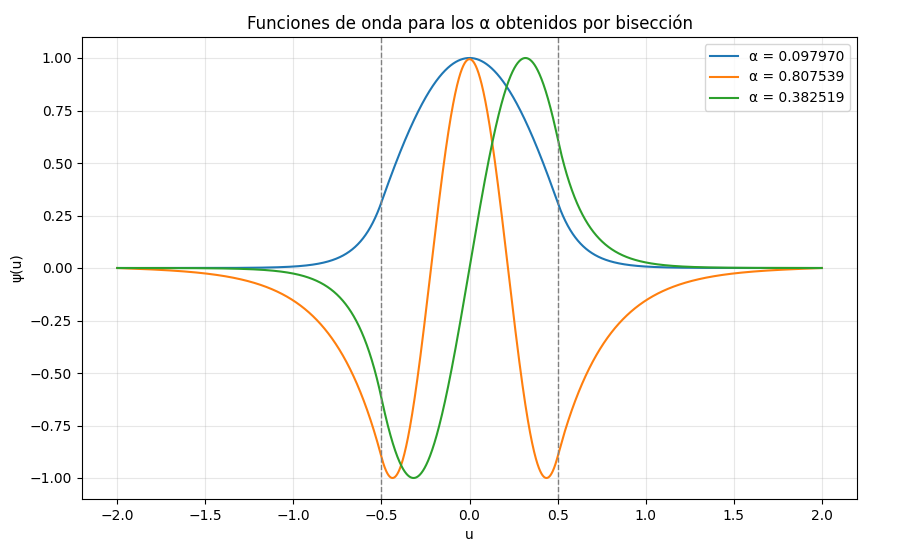
\includegraphics[width=0.8\textwidth]{imagenes/DifFIn.png}
    \caption{Funciones de onda obtenidas del método de diferencias finitas.}
    \label{fig:DifFIn}
\end{figure}

\subsection{Método de Numerov}

\section{Conclusiones}
El método de Numerov demostró una convergencia significativamente más rápida que el de diferencias finitas debido a su mayor orden de aproximación[cite: 222, 371]. La elección del paso de integración $\Delta x$ resultó crítica para evitar la divergencia en el método de disparo[cite: 161].

\section{Bibliografía}
\begin{enumerate}
    \item Palencia, E., Ramon, C., Trapote, A. \textit{Pozo de Potencial}. Física Atómica, Nuclear y de Partículas[cite: 4].
    \item Palencia, E., Ramon, C., Trapote, A. \textit{Método de Numerov - Átomos}. Física Atómica, Nuclear y de Partículas[cite: 192].
\end{enumerate}

\end{document}